\documentclass[11pt,a4paper]{report}
\usepackage[utf8]{inputenc}
\usepackage{amsmath}
\usepackage{amsfonts}
\usepackage{amssymb}
\usepackage{amsthm}
\usepackage{geometry}
\geometry{margin=1in}
\usepackage{lineno} 
\theoremstyle{definition}
\newtheorem{definition}{Definition}
\newtheorem{example}{Example}
\newtheorem{property}{Property}
\newtheorem{remark}{Remark}
\newtheorem{theorem}{Theorem}

\providecommand{\promed}[1]{{\mathbb{E}}\left\lbrace #1\right\rbrace}
\providecommand{\ve}[1]{{\boldsymbol{#1}}}
\providecommand{\mat}[1]{{\pmb{#1}}}
\newcommand{\Real}{\mathbb{R}}
\newcommand{\N}{\mathbb{N}}

\usepackage{tikz}
\usetikzlibrary{positioning, arrows.meta}
\begin{document}
%\linenumbers
\section*{\centering Estimation of Wideband PSD Parameters }

\begin{center}
	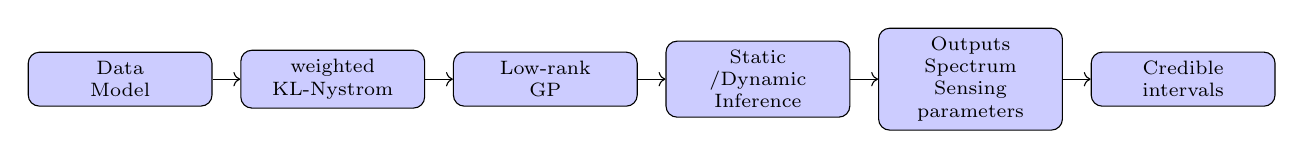
\begin{tikzpicture}[node distance=2.7cm]
		
		\tikzstyle{process} = [rectangle, draw, fill=blue!20, rounded corners, text width=2.1cm, align=center, font=\scriptsize]
		
		% Define nodes
		\node[process] (first) {Data \\ Model};
		\node[process, right of=first] (second) {weighted \\KL-Nystrom};
		\node[process, right of=second] (third) {Low-rank\\ GP};
		\node[process, right of=third] (fourth) {Static\\ /Dynamic\\ Inference};
		\node[process, right of=fourth] (fifth) {Outputs\\
		Spectrum Sensing\\ parameters};
		\node[process, right of=fifth] (sixth) {Credible\\intervals};
		
		% Draw arrows
		\draw[->] (first) -- (second);
		\draw[->] (second) -- (third);
		\draw[->] (third) -- (fourth);
		\draw[->] (fourth) -- (fifth);
		\draw[->] (fifth) -- (sixth);
		
	\end{tikzpicture}
	
\end{center}

\subsection*{PSD Estimation via KL + GP}
\paragraph{Data model.}
Let $\{f_i\}_{i=1}^M$ be a frequency grid with quadrature weights $\{w_i\}_{i=1}^M$ (w.r.t.\ the Lebesgue measure unless otherwise specified). For wideband spectrum sensing, the default choice is a uniform grid of weights since FFT-based measurements naturally produce uniform frequency grids with spacing 
$\Delta f$, that is $w_i{=}\Delta f,\,\forall i$. This avoids scaling 
errors in high-dimensional problems and ensures $\sum_{i=1}^M w_i {=} M \Delta f {=} B_{\text{total}}$. 
Trapezoidal weights, i.e., $w_i {=} (f_{i+1} - f_{i-1})/2$ with boundary adjustments, 
are preferred when high accuracy is needed for narrow-band features or non-uniform grids.

Over a given frequency grid, assume \(\ve{y}\) be a linearized/averaged surrogate of PSD data \({\mid} X(f){\mid}^{2}\), then the observed subsampled measurements are modelled as:
\begin{align}
	\ve{y} = \boldsymbol{\varTheta}\,\ve{s} + \boldsymbol{\varepsilon}, 
	\quad 	\ve{y} \in \mathbb{R}^N, \qquad \boldsymbol{\varepsilon} \sim \mathcal{N}(\mathbf{0}, \boldsymbol{ \varSigma}_\varepsilon),
\end{align}
where $\ve{s} {\in} \mathbb{R}^{M}$ is the (unknown) PSD over the frequency grid, $\boldsymbol{\varTheta}{\in} \mathbb{R}^{N \times M}$ is a known linear sampling/sensing operator (\(N {\le} M\) -- subsampling), and $\boldsymbol{ \varepsilon}{\sim} \mathcal{N}(0,\varSigma_\epsilon)$ is the noise term, having covariance\(,\varSigma_\epsilon{\in}\Real^{N\times N}\). A common special case is homoscedastic noise with $ \varSigma_\epsilon{=}\sigma^{^2} \mat{I}_N$.

\paragraph{KL basis construction.}
Choose a positive definite kernel $k_f {:} \mathcal{F}\times \mathcal{F}{\to} \mathbb{R}$ on frequency.
Form the weighted Gram matrix with entries:
\begin{align}
	\mat{K}_w[{ij}] = k_f(f_i, f_j)\,\sqrt{w_i w_j}, \quad i,j=1,\dots,M.
\end{align}
Compute its eigendecomposition (retain $R {\ll} M$ dominant modes):
\begin{align}
	\mat{K}_w \,\ve{v}_n = \lambda_n \,\ve{v}_n,\quad\lambda_1{ \ge} \cdots {\ge} \lambda_R {>} 0, 
	\quad n=1,\dots,R
\end{align}
Define discrete eigenfunctions on the grid
\begin{align}
	\phi_n(f_i) \approx {\ve{v}_n[i]}/{\sqrt{w_i}}, 
	\qquad i=1,\dots,M.
\end{align}
For off-grid evaluation $f{\in} \mathcal{F}$ (Nyström extension):
\begin{align}
	\phi_n(f) \approx \frac{1}{\lambda_n} \sum_{j=1}^{M} k_f(f, f_j)\, w_j\, \phi_n(f_j).
\end{align}

\paragraph{KL feature matrix and low-rank field model.}
Define the KL feature matrix $\boldsymbol{\Phi}_{\!\mathrm{KL}}{\in}\mathbb{R}^{M\times R}$ by its entries
\begin{align}
	(\boldsymbol{\Phi}_{\!\mathrm{KL}})_{in} := \sqrt{\lambda_n}\,\phi_n(f_i),
	\qquad i=1,\dots,M,\; n=1,\dots,R.
\end{align}
Approximate the PSD on the grid by the rank-$R$ KL expansion
\begin{align}
	\ve{s} \approx \boldsymbol{\Phi}_{\!\mathrm{KL}}\,\boldsymbol{\xi},
	\qquad \boldsymbol{\xi}\in\mathbb{R}^R,
\end{align}
with prior $\boldsymbol{\xi}{\sim}\mathcal{N}(\ve{0},\mat{I}_R)$.
This induces the (approximate) truncated Mercer/KL covariance on $\ve{s}$:
\begin{align}
	\mathrm{Cov}(\ve{s})
	\approx \boldsymbol{\Phi}_{\!\mathrm{KL}}\boldsymbol{\Phi}_{\!\mathrm{KL}}^\top
	= \sum_{n=1}^R \lambda_n\,\boldsymbol{\phi}_n \boldsymbol{\phi}_n^\top,
\end{align}
where $\boldsymbol{\phi}_n := [\phi_n(f_1),\dots,\phi_n(f_M)]^\top\in\mathbb{R}^M$.
The measurement model becomes
\begin{align}
	\ve{y} \approx \mat{\varTheta}\boldsymbol{\Phi}_{\!\mathrm{KL}}\,\boldsymbol{\xi} + \ve{\varepsilon},
	\qquad \ve{\varepsilon}\sim\mathcal{N}(\ve{0},\boldsymbol{\varSigma}_{\varepsilon}).
\end{align}

\paragraph{[Single-window] Static Bayesian linear regression.}
Let $\mathbf{A} {:=} \boldsymbol{\varTheta}\,\boldsymbol{\Phi}_{\!\mathrm{KL}} {\in} \mathbb{R}^{N\times R}$ so that $\ve{y} {=} \mat{A}\,\boldsymbol{\xi} {+} \boldsymbol{\varepsilon}$.
With $\boldsymbol{\xi} {\sim} \mathcal{N}(\ve{0}, \mat{I}_R)$ and $\boldsymbol{\varepsilon}{\sim} \mathcal{N}(\mathbf{0},\boldsymbol{ \varSigma}_\varepsilon)$, the posterior is
\begin{subequations}
\begin{align}
	\boldsymbol{ \varSigma}_{\xi|y} &= \Big(\mat{I}_R + \mat{A}^\top \boldsymbol{ \varSigma}_\varepsilon^{-1} \mat{A}\Big)^{-1}, \\
	\boldsymbol{\mu}_{\xi|y} &= \boldsymbol{ \varSigma}_{\xi|y}\,\mat{A}^\top \boldsymbol{ \varSigma}_\varepsilon^{-1} \ve{y}.
\end{align}
\end{subequations}
Within a single window, the PSD posterior (on the grid) is Gaussian with
\begin{subequations}
\begin{align}
	\boldsymbol{\mu}_{s|y} &= \boldsymbol{\Phi}_{\!\mathrm{KL}} \,\boldsymbol{\mu}_{\xi|y}, \\
	\boldsymbol{ \varSigma}_{s|y} &= \boldsymbol{\Phi}_{\!\mathrm{KL}} \,\boldsymbol{ \varSigma}_{\xi|y}\, \boldsymbol{\Phi}_{\!\mathrm{KL}}^\top.
\end{align}
\end{subequations}

\paragraph{[Multiple-windows] Dynamic GP prior on coefficients.}
For windows $t{=}1,\dots,T$, let $\ve{y}_t {=} \boldsymbol{\varTheta}_t\,\ve{s}_t + \boldsymbol{\varepsilon}_t$ and assume
$\ve{s}_t {\approx} \boldsymbol{\Phi}_{\!\mathrm{KL}} \boldsymbol{\xi}_t$ with $\boldsymbol{\xi}_t {\in} \mathbb{R}^{R}$.

Place independent GP priors across time on coefficients:
\begin{align}
	\xi_n(\cdot) \sim \mathcal{GP}(0, k_n(\cdot,\cdot)), \qquad n=1,\dots,R,
\end{align}
e.g., Matérn kernels ($\nu \in \{1/2, 3/2, 5/2\}$).

Use state-space realizations for scalable inference. Particularly, for $\nu{=}1/2$ (Ornstein--Uhlenbeck state-space form), the discrete-time model for step $\Delta t_t$ is
\begin{subequations}
\begin{align}
	\xi_{n,t} &= a_{n,t}\,\xi_{n,t-1} + \eta_{n,t}, 
	\quad a_{n,t} = e^{-\alpha_n \Delta t_t}, \\
	\eta_{n,t} &\sim \mathcal{N}\!\Big(0,\, q_n \frac{1-e^{-2\alpha_n \Delta t_t}}{2\alpha_n}\Big),
\end{align}
\end{subequations}
The stationary initial prior is \(\xi_{n,1} {\sim} \mathcal{N}(0, q_n/(2\alpha_n)), \) with hyperparameters $\alpha_n, q_n {>}0$. This state-space representation enables efficient $\mathcal{O}(TR^{2})$ inference via Kalman filtering/smoothing 

In the following case of $\nu{\in}\{3/2,5/2\}$, use standard $p$-dimensional Markov state embeddings with known $(\mat{F}_n, \mat{L}_n, \mat{Q}_n)$ (omitted for brevity).

The observation equation is
\begin{align}
	\ve{y}_t = \mat{H}_t \,\boldsymbol{\xi}_t + \boldsymbol{\varepsilon}_t,
	\qquad \mat{H}_t := \boldsymbol{\varTheta}_t\,\boldsymbol{\Phi}_{\!\mathrm{KL}}, 
	\qquad \boldsymbol{\varepsilon}_t \sim \mathcal{N}(\ve{0}, \boldsymbol{ \varSigma}_{\varepsilon,t}).
\end{align}
Run a $R$-dimensional Kalman filtering with diaganonal transition $\mat{A}{=}\operatorname{diag}(a_{n,t})$ and diagonal process noise $\mat{Q}_t{=}\operatorname{diag}(\cdot)$, using Rauch--Tung--Striebel smoothing across $t$ and across modes $n$, and producing smoothed $\boldsymbol{\mu}_{\xi|y, t}$ and $\boldsymbol{ \varSigma}_{\xi|y, t}$, and reconstruct
\begin{align}
	\boldsymbol{\mu}_{s|y, t} = \mathbf{\Phi}_{\!\mathrm{KL}} \,\boldsymbol{\mu}_{\xi|y, t}, 
	\qquad 
	\boldsymbol{ \varSigma}_{s|y, t} = \mathbf{\Phi}_{\!\mathrm{KL}} \,\boldsymbol{ \varSigma}_{\xi|y, t}\, \mathbf{\Phi}_{\!\mathrm{KL}}^\top.
\end{align}

Mostly, state-space representations reformulate GP regression using Kalman filtering theory, achieving $\mathcal{O}(n)$ complexity for linear-time Markovian processes (plus the cost to handle \(	\boldsymbol{ \varSigma}_{\epsilon, t}\)). 

\subsection*{Outputs: Spectral Parameter Estimation}

\paragraph*{Spectral parameter estimation from the reconstructed PSD.} Let $\{f_i\}_{i=1}^M$ be the frequency grid with quadrature weights $\{w_i\}_{i=1}^M$ (for a uniform grid, $w_i=\Delta f$). From the KL+GP inference, assume the (approx.) Gaussian posterior
\[
\ve{s}\mid \ve{y}\;\sim\;\mathcal{N}\!\big(\,\boldsymbol{\mu}_{s\mid y},\,\boldsymbol{\varSigma}_{s\mid y}\big),
\qquad
\mu_{s\mid y,i}:=\boldsymbol{\mu}_{s\mid y}[i],\quad
\sigma_{s\mid y,i}:=\sqrt{\boldsymbol{\varSigma}_{s\mid y}[i,i]}.
\]
All feature computations assume PSD values are in \emph{linear} power units (not dB); if inputs are in dB, convert via $s^{\mathrm{lin}}=10^{s^{\mathrm{dB}}/10}$ before applying the definitions below.

\begin{description}
\item[PSD credible bands]\;

\textit{Band statistic:} Let $B {\subset} \{1,\dots,M\}$ be an index set (band), and define a linear band statistic
\(p_B {:=} \ve{c}_B^\top \ve{s}, \; \ve{c}_B{ \in} \mathbb{R}^M.\) Two common choices for $\ve{c}_B$ are:
\begin{align*}
	\text{(Average PSD over $B$)}\quad
	c_B[i] &=
	\begin{cases}
		\dfrac{w_i}{\sum_{j \in B} w_j}, & i \in B,\\[6pt]
		0, & \text{otherwise,}
	\end{cases}
	\\[6pt]
	\text{(Total band power over $B$)}\quad
	c_B[i] &=
	\begin{cases}
		w_i, & i \in B,\\[4pt]
		0, & \text{otherwise.}
	\end{cases}
\end{align*}
The average PSD choice, $p_B$, has units of power/Hz; the total power choice, $p_B$, has units of power. Note that $\sum_{i=1}^M w_i s_i$ approximates $\int s(f)\,df$.

\textit{Pointwise PSD posterior and credible intervals.}
For a grid index $i$,
\[
s_i \mid \ve{y} \sim \mathcal{N}\!\big(\mu_{s\mid y,i},\, \sigma^2_{s\mid y,i}\big), 
\quad
\mu_{s\mid y,i} := \mu_{s\mid y}[i], 
\quad
\sigma_{s\mid y,i} := \sqrt{\varSigma_{s\mid y}[i,i]}.
\]
A $(1-\alpha)$ pointwise credible interval is
\[
\mu_{s\mid y,i} \;\pm\; z_{1-\alpha/2}\,\sigma_{s\mid y,i},
\quad
z_p := \Psi^{-1}(p),
\]
where $\Psi(\cdot)$ is the standard normal CDF.

\textit{Band statistic posterior and credible intervals.}
Because $p_B$ is linear in $\ve{s}$, under the Gaussian posterior for $\ve{s}$ we have
\[
p_B \mid \ve{y} \sim \mathcal{N}\!\big(\mu_B,\, \sigma_B^2\big),
\quad
\mu_B := \ve{c}_B^\top \mu_{s\mid y},
\quad
\sigma_B^2 := \ve{c}_B^\top \varSigma_{s\mid y}\, \ve{c}_B.
\]
A $(1-\alpha)$ credible interval for $p_B$ is
\(
\mu_B \;\pm\; z_{1-\alpha/2}\,\sigma_B.
\)

\item[{Occupancy probabilities (per-bin and per-band).}]
Given thresholds $\tau_i$ (per-bin) and $\tau_B$ (per-band), the posterior occupancy probability is defined as:
\begin{align*}
\pi_i :=	\Pr\!\big(s_i > \tau_i \mid \ve{y}\big) 
	&= 1 - \Psi\!\left(\frac{\tau_i - \mu_{s\mid y,i}}{\sigma_{s\mid y,i}}\right),\\[4pt]
\pi_B :=	\Pr\!\big(p_B > \tau_B \mid \ve{y}\big) 
	&= 1 - \Psi\!\left(\frac{\tau_B - \mu_B}{\sigma_B}\right).
\end{align*}
\textit{Decision rule:} declare bin $i$ (or band $B$) occupied if the corresponding posterior probability \(\pi_i {\in}[0,1]\) exceeds a target (e.g., $0.5$ or another application-driven threshold).

\textit{Threshold calibration under noise-only (example).}
Let $s_{\mathrm{nf}}$ denote the (approximately white) \emph{noise-floor PSD level} (in linear units, e.g., W/Hz) under a noise-only reference; $s_{\mathrm{nf}}$ is a property of the background spectrum $\ve{s}$ and should not be confused with the \emph{measurement-error} covariance $\boldsymbol{\varSigma}_{\varepsilon}$ in $\ve{y}{=}\boldsymbol{\varTheta}\ve{s}{+}\boldsymbol{\varepsilon}$.
For the average-PSD statistic over $B$ with $|B|$ bins, under a noise-only reference model with (white) noise PSD $s_{\mathrm{nf}}$ and an independent-bin normal approximation,
\[
\tau_B 
\;\approx\; s_{\mathrm{nf}}\!\left(\,1 + \sqrt{\frac{2}{|B|}}\,Q^{-1}\!\big(P_{\mathrm{fa}}\big)\right),
\qquad
Q(x) := 1 - \Psi(x),
\]
which yields $\Pr(\text{false alarm}) {\approx} P_{\mathrm{fa}}$.
A consistent per-bin choice is obtained by setting $|B|{=}1$:
\[
\tau_i \;\approx\; s_{\mathrm{nf}}\!\left(\,1 + \sqrt{2}\,Q^{-1}\!\big(P_{\mathrm{fa},i}\big)\right).
\]
Calibrate analogously for the total-power statistic if that definition of $\mathbf{c}_B$ is used.

\textit{plug-in rule:} Replace $\pi_i\ge\pi_0$ by $\mu_{s\mid y,i}>\tau_i$.

\item[{Peak frequency.}]
A simple (single-peak) estimate is
\[
i_\star \;:=\; \arg\max_{1\le i\le M}\ \mu_{s\mid y,i},
\qquad
\widehat{f}_{\mathrm{peak}} \;:=\; f_{i_\star}.
\]
If you want the peak \emph{within} occupied bins, use
$
i_\star := \arg\max_{i\in\widehat{\mathcal{O}}}\mu_{s\mid y,i}
$
(when $\widehat{\mathcal{O}}\neq\emptyset$).

\item[{Spectral centroid (center frequency).}]
The power-weighted centroid (optionally restricted to occupied bins) is
\[
\widehat{f}_{c}
\;:=\;
{\sum\limits_{i\in\widehat{\mathcal{O}}} f_i\, w_i\, \mu_{s\mid y,i}}
\big{/}{\sum\limits_{i\in\widehat{\mathcal{O}}} w_i\, \mu_{s\mid y,i}},
\qquad
\text{(use } \widehat{\mathcal{O}}=\{1,\dots,M\}\text{ if no occupancy gating).}
\]

\item[{Occupied bandwidth.}]
If $\widehat{\mathcal{O}}\neq\emptyset$, define the occupied support endpoints
\[
\widehat{f}_{\min}:=\min_{i\in\widehat{\mathcal{O}}} f_i,
\qquad
\widehat{f}_{\max}:=\max_{i\in\widehat{\mathcal{O}}} f_i,
\qquad
\widehat{B}_{\mathrm{occ}}:=\widehat{f}_{\max}-\widehat{f}_{\min}.
\]
For multiple disjoint emitters, compute \emph{connected components} of $\widehat{\mathcal{O}}$
(contiguous index runs) to obtain $\{\widehat{B}_{\mathrm{occ}}^{(k)}\}_k$ and peaks per component.

\smallskip
\noindent\emph{Uncertainty-aware alternative (expected occupied bandwidth).}
For a uniform grid ($w_i=\Delta f$), a soft estimate is
\[
\promed{B_{\mathrm{occ}}\mid \ve{y}} \;\approx\; \sum_{i=1}^M \pi_i\,\Delta f
\quad
\text{(or }\sum_i \pi_i w_i\text{ for non-uniform grids).}
\]

\item[{SNR}] from reconstructed PSD (noise-floor estimated from unoccupied bins).
Let $\pi_N$ be a small cutoff (e.g., $\pi_N=0.1$) and define a noise-bin set
\[
\widehat{\mathcal{N}} \;:=\; \{\,i:\ \pi_i\le \pi_N\,\}.
\]
Estimate the (approximately white) noise floor (PSD level) by a weighted average
\[
\widehat{s}_{n} \;:=\;
{\sum\limits_{i\in\widehat{\mathcal{N}}} w_i\, \mu_{s\mid y,i}}\big{/}
{\sum\limits_{i\in\widehat{\mathcal{N}}} w_i}.
\]
Then estimate \emph{signal power above the noise floor} over occupied bins as
\[
\widehat{P}_{\mathrm{sig}}
\;:=\;
\sum_{i\in\widehat{\mathcal{O}}} w_i\,\big(\mu_{s\mid y,i}-\widehat{s}_n\big)_+,
\qquad (x)_+:=\max(x,0),
\]
and the corresponding noise power in the same support as
\[
\widehat{P}_{\mathrm{noise}}
\;:=\;
\widehat{s}_{n}\sum_{i\in\widehat{\mathcal{O}}} w_i.
\]
Finally, define the SNR (linear and dB):
\[
\widehat{\mathrm{SNR}}
\;:=\;
\frac{\widehat{P}_{\mathrm{sig}}}{\widehat{P}_{\mathrm{noise}}},
\qquad
\widehat{\mathrm{SNR}}_{\mathrm{dB}}
\;:=\;
10\log_{10}\big(\widehat{\mathrm{SNR}}\big).
\]
If a calibrated noise-floor PSD level $s_{\mathrm{nf}}$ is already available (e.g., from hardware calibration or empty-band measurements), the value $\widehat{s}_n:=s_{\mathrm{nf}}$ can be set and skip $\widehat{\mathcal{N}}$.


\item[{(0)Credible intervals for these features.}]
To propagate posterior uncertainty, draw samples
$\ve{s}^{(m)}{\sim}\mathcal{N}(\boldsymbol{\mu}_{s\mid y},\mat{\Sigma}_{s\mid y})$
(or from the KL-latent posterior) and compute
\[\{f_{\mathrm{peak}}^{(m)}, f_c^{(m)}, B_{\mathrm{occ}}^{(m)}, \mathrm{SNR}^{(m)}\}_{m=1}^M
\]
Report empirical quantiles (e.g., $2.5\%-97.5\%$) as credible intervals.
\end{description}
%
%\paragraph{Hyperparameters and learning.}
%Kernel hyperparameters for $k_f$ (frequency), dynamic priors $k_n$ (time), and noise 
%$\boldsymbol{\varSigma}_\varepsilon$ can be learned by maximizing the (marginal) likelihood or via cross-validation.
%
%\subparagraph{Static model: marginal likelihood optimization.}
%In the static model with $\boldsymbol{\xi}\sim\mathcal{N}(\ve{0},\mat{I})$, the log marginal likelihood is
%\begin{align}
%	\log p(\ve{y}\mid\boldsymbol{\theta}) 
%	= -\tfrac{1}{2}\ve{y}^\top \big(\mat{A}\mat{A}^\top + \boldsymbol{\varSigma}_\varepsilon\big)^{-1}\ve{y}
%	-\tfrac{1}{2}\log\big|\mat{A}\mat{A}^\top + \boldsymbol{\varSigma}_\varepsilon\big|
%	-\tfrac{N}{2}\log(2\pi),
%\end{align}
%where $\boldsymbol{\theta}$ collects all hyperparameters: frequency kernel parameters (e.g., lengthscale $\ell_f$, variance $\sigma_f^2$), and noise level $\sigma_\varepsilon^2$.
%
%\textbf{Optimization strategy:}
%Use gradient-based methods (L-BFGS-B, Adam) with automatic differentiation. The gradient w.r.t.\ $\theta_k$ is:
%\begin{align}
%	\frac{\partial \log p(\ve{y}\mid\boldsymbol{\theta})}{\partial \theta_k}
%	= \tfrac{1}{2}\mathrm{tr}\Big[\big(\boldsymbol{\alpha}\boldsymbol{\alpha}^\top - \mat{C}^{-1}\big)\frac{\partial \mat{C}}{\partial \theta_k}\Big],
%\end{align}
%where $\mat{C} = \mat{A}\mat{A}^\top + \boldsymbol{\varSigma}_\varepsilon$ and $\boldsymbol{\alpha} = \mat{C}^{-1}\ve{y}$.
%
%\textbf{Computational cost:} Each likelihood evaluation requires $\mathcal{O}(N^3)$ for Cholesky decomposition or $\mathcal{O}(NR^2)$ using the Woodbury identity:
%\begin{align}
%	\mat{C}^{-1} = \boldsymbol{\varSigma}_\varepsilon^{-1} - \boldsymbol{\varSigma}_\varepsilon^{-1}\mat{A}\big(\mat{I}_R + \mat{A}^\top\boldsymbol{\varSigma}_\varepsilon^{-1}\mat{A}\big)^{-1}\mat{A}^\top\boldsymbol{\varSigma}_\varepsilon^{-1}.
%\end{align}
%
%\subparagraph{Initialization guidelines.}
%\textbf{Frequency kernel $k_f$:}
%\begin{itemize}
%	\item \textit{Lengthscale} $\ell_f$: Initialize to capture expected correlation bandwidth. For Matérn kernels, use $\ell_f \approx 0.1 \times B_{\text{total}}$ (10\% of total bandwidth) as a starting point. For narrowband signals, use smaller values ($\ell_f \approx 0.01 \times B_{\text{total}}$).
%	
%	\item \textit{Variance} $\sigma_f^2$: Initialize to the empirical variance of a rough PSD estimate (e.g., from periodogram): $\sigma_f^2 \approx \mathrm{Var}(\hat{\ve{s}}_{\text{init}})$.
%	
%	\item \textit{Smoothness} $\nu$ (for Matérn): Start with $\nu = 3/2$ (once differentiable) for typical RF spectra. Use $\nu = 5/2$ for smoother spectra, $\nu = 1/2$ for rough/discontinuous.
%\end{itemize}
%
%\textbf{Noise variance} $\sigma_\varepsilon^2$:
%Initialize from hardware specs or empirical noise floor:
%\begin{align}
%	\sigma_\varepsilon^2 \approx k_B T B_{\text{sensor}} F_{\text{noise}},
%\end{align}
%where $k_B$ is Boltzmann's constant, $T$ is temperature, $B_{\text{sensor}}$ is sensor bandwidth, and $F_{\text{noise}}$ is the noise figure.
%
%\textbf{Temporal kernel $k_n$ (for dynamic model):}
%\begin{itemize}
%	\item \textit{Lengthscale} $\ell_t$ or $1/\alpha_n$: Initialize to expected correlation time. For slowly-varying spectra (e.g., cognitive radio), use $\ell_t \approx 10\times T_{\text{window}}$. For rapidly-varying (e.g., frequency-hopping), use $\ell_t \approx T_{\text{window}}$.
%	
%	\item \textit{Variance} $q_n$: Initialize to allow moderate temporal variation: $q_n \approx 0.1$ (relative to unit-variance prior on $\xi$).
%\end{itemize}
%
%\subparagraph{Identifiability and constraints.}
%\textbf{Key identifiability issue:} The frequency kernel variance $\sigma_f^2$ and the KL coefficient prior variance (fixed at 1) interact through the eigenvalues $\{\lambda_n\}$. Similarly, temporal kernel variance $q_n$ trades off with the frequency kernel.
%
%\textbf{Recommended constraints:}
%\begin{itemize}
%	\item \textbf{Normalize frequency kernel:} Fix $k_f(0,0) = 1$ (unit variance at origin) to avoid redundancy with coefficient scaling. Equivalently, constrain $\sigma_f^2 = 1$ and absorb signal power into the data likelihood.
%	
%	\item \textbf{Mode-specific temporal variances:} Allow different $q_n$ for each KL mode $n$, but regularize via a hierarchical prior:
%	\begin{align}
%		q_n \sim \text{InverseGamma}(a_0, b_0),
%	\end{align}
%	with $a_0 = b_0 = 1$ (weak prior encouraging $q_n \approx 1$).
%	
%	\item \textbf{Noise floor constraint:} Enforce $\sigma_\varepsilon^2 \geq \sigma_{\min}^2$ based on hardware noise floor to prevent overfitting.
%\end{itemize}
%
%\subparagraph{Cross-validation strategy.}
%For finite datasets with $T$ windows, use \textbf{time-series cross-validation}:
%
%\textbf{Expanding window CV:}
%\begin{enumerate}
%	\item Split data into training windows $\{1, \ldots, t_{\text{train}}\}$ and validation $\{t_{\text{train}}+1, \ldots, t_{\text{train}}+t_{\text{val}}\}$.
%	\item Train model on training set, predict on validation set.
%	\item Compute validation score: negative log predictive density (NLPD):
%	\begin{align}
%		\text{NLPD} = -\sum_{t=t_{\text{train}}+1}^{t_{\text{train}}+t_{\text{val}}} \log p(\ve{y}_t \mid \ve{y}_{1:t-1}, \boldsymbol{\theta}).
%	\end{align}
%	\item Increment $t_{\text{train}}$ and repeat, averaging scores across folds.
%\end{enumerate}
%
%\textbf{Alternative: leave-future-out CV.}
%Fix training window size, slide forward in time, always predict future observations.
%
%\subparagraph{Multi-scale optimization.}
%For large problems, use a \textbf{coarse-to-fine} strategy:
%\begin{enumerate}
%	\item \textbf{Stage 1 (coarse grid):} Learn hyperparameters on a downsampled frequency grid ($M' \ll M$) to get rough estimates quickly.
%	
%	\item \textbf{Stage 2 (full grid):} Refine hyperparameters on the full grid using Stage 1 values as initialization.
%	
%	\item \textbf{Stage 3 (mode-specific):} Fix frequency kernel, optimize temporal parameters $\{\alpha_n, q_n\}$ per mode independently via mode-specific likelihoods.
%\end{enumerate}
%
%\subparagraph{Practical recipe.}
%\begin{enumerate}
%	\item \textbf{Initialize:} Use domain knowledge (bandwidth correlations, expected smoothness, noise floor).
%	
%	\item \textbf{Optimize frequency kernel:} Maximize marginal likelihood on a single representative window, holding noise variance fixed.
%	
%	\item \textbf{Optimize noise variance:} With frequency kernel fixed, optimize $\sigma_\varepsilon^2$ (or learn per-window if heteroscedastic).
%	
%	\item \textbf{Optimize temporal kernels:} For the dynamic model, use expanding-window CV to tune $\{\alpha_n, q_n\}$.
%	
%	\item \textbf{Joint refinement:} Optionally, perform joint optimization of all parameters, using the above as initialization.
%	
%	\item \textbf{Validate:} Check that learned parameters are physically reasonable (e.g., $\ell_f$ matches expected signal bandwidths, $\sigma_\varepsilon^2$ aligns with SNR).
%\end{enumerate}
%
%\subparagraph{Diagnostic checks.}
%\begin{itemize}
%	\item \textbf{Residual analysis:} Standardized residuals $\ve{r} = \boldsymbol{\varSigma}_\varepsilon^{-1/2}(\ve{y} - \mat{A}\boldsymbol{\mu}_{\xi|y})$ should be approximately $\mathcal{N}(\ve{0}, \mat{I})$. Check via Q-Q plots.
%	
%	\item \textbf{Predictive checks:} Simulate data from the posterior predictive $p(\ve{y}^* \mid \ve{y})$ and compare to held-out observations. Large discrepancies indicate model misspecification.
%	
%	\item \textbf{Hyperparameter stability:} Repeat optimization from multiple random initializations. If results vary significantly, consider stronger priors or more data.
%\end{itemize}
%\paragraph{Complexity and benefits.}
%The KL truncation yields rank-$R$ features and reduces complexity:
%\begin{itemize}
%	\item Static window (posterior of $\boldsymbol{\xi}$): forming and solving involves $\mathcal{O}(NR^2 + R^3)$.
%	\item Streaming with Kalman: per step $\mathcal{O}(NR^2 + R^3)$ (often dominated by $\mathbf{H}_t$ multiplies and a size-$R$ Riccati update).
%	\item Nyström eigendecomposition on $M$-grid: typically $\mathcal{O}(M^3)$ once, then reused; for large $M$, randomized/Nyström acceleration may be used.
%\end{itemize}
%Benefits include robustness at low SNR, principled uncertainty quantification, and efficient sub-Nyquist recovery driven by low-rank spectral structure.
%
%\paragraph{Implementation notes.}
%\begin{itemize}
%	\item {Weight consistency checklist.}
%	\begin{itemize}
%		\item Verify $\sum_{i=1}^M w_i = B_{\text{total}}$ (total bandwidth)
%		\item Use identical $\{w_i\}$ in Gram matrix construction, eigenfunction definition, 
%		Nyström extension, and band power calculation
%		\item For uniform grid: $w_i = \Delta f = B_{\text{total}}/M$
%		\item For non-uniform grid: $w_i = (f_{i+1} - f_{i-1})/2$ with boundary corrections
%		\item Test orthonormality: $\sum_i \phi_n(f_i) \phi_m(f_i) w_i \approx \delta_{nm}$
%		\item Verify Nyström: $|\phi_n(f_k) - (1/\lambda_n) \sum_j k_f(f_k,f_j) w_j \phi_n(f_j)| < \epsilon$
%	\end{itemize}
%	\item Choose $R$ via cumulative variance: $\sum_{n=1}^R \lambda_n / \sum_{n=1}^M \lambda_n \in [0.95,\,0.99]$.
%	\item Ensure weighted inner products in projections and Nyström consistency to avoid scaling errors.
%	\item Composite kernels on frequency (e.g., Matérn + periodic) can capture narrowband and cyclostationary patterns.
%	\item \textbf{Sub-Nyquist Recovery Conditions.} The wideband PSD estimation framework enables recovery under sub-Nyquist sampling when the following key conditions are satisfied:
%	
%	\textbf{Low-Rank Spectral Structure:}
%	The PSD can be well-approximated by a truncated Karhunen-Loève (KL) expansion:
%	\begin{equation}
%		\mathbf{s} \approx \boldsymbol{\Phi}_{\text{KL}} \boldsymbol{\xi}, \quad \boldsymbol{\xi} \in \mathbb{R}^R
%	\end{equation}
%	where $R \ll M$ (the rank is much smaller than the number of frequency bins).
%	
%	\textbf{Kernel Expressivity Condition:}
%	The chosen frequency kernel $k_f$ must be sufficiently expressive to capture the spectral characteristics, with appropriate parameters:
%	\begin{itemize}
%		\item Lengthscale: $\ell_f \approx 0.1 \times B_{\text{total}}$ for typical signals
%		\item Smoothness parameter (for Matérn): $\nu \in \{1/2, 3/2, 5/2\}$ matching signal regularity
%	\end{itemize}
%	
%	\textbf{Sampling Operator Requirements:}
%	The linear sampling/sensing operator $\boldsymbol{\Theta} \in \mathbb{R}^{N \times M}$ must satisfy:
%	\begin{itemize}
%		\item Sub-Nyquist condition: $N < M$
%		\item Sufficient incoherence with the KL basis
%		\item Adequate restricted isometry properties when combined with the KL basis
%	\end{itemize}
%	
%	\textbf{Measurement SNR Condition:}
%	The noise covariance $\boldsymbol{\Sigma}_\varepsilon$ must permit reliable signal detection:
%	\begin{equation}
%		\sigma^2_\varepsilon < \text{min signal power of interest}
%	\end{equation}
%	
%	\textbf{KL Mode Selection Criterion:}
%	The retained KL modes should capture most of the signal variance:
%	\begin{equation}
%		\frac{\sum_{n=1}^R \lambda_n}{\sum_{n=1}^M \lambda_n} \in [0.95, 0.99]
%	\end{equation}
%	
%	\textbf{Effective Dimensionality Reduction:}
%	The computational complexity benefits are realized when:
%	\begin{equation}
%		O(NR^2 + R^3) \ll O(NM^2 + M^3)
%	\end{equation}
%	which is satisfied when $R \ll M$ and the recovery conditions above hold.
%\end{itemize}
%
%\textbf{Next Steps for Implementation}
%
%The mathematical framework presented in the document provides a solid foundation for wideband PSD estimation and occupancy detection. The following steps outline a structured implementation approach:
%
%\begin{enumerate}
%	\item \textbf{Core Algorithm Implementation}
%	\begin{itemize}
%		\item Implement weighted Gram matrix construction: $[K_w]_{ij} = k_f(f_i, f_j)\sqrt{w_i w_j}$
%		\item Develop efficient eigendecomposition for KL basis extraction: $K_w v_n = \lambda_n v_n$
%		\item Construct the KL feature matrix: $\Phi_{\text{KL}} = \sqrt{\lambda_n}\phi_n(f_i)$
%		\item Implement the posterior inference engine:
%		\begin{subequations}
%		\begin{align}
%			\mu_{s|y} &= \Phi_{\text{KL}}\mu_{\xi|y}\\
%			\Sigma_{s|y} &= \Phi_{\text{KL}}\Sigma_{\xi|y}\Phi^{\top}_{\text{KL}}
%		\end{align}
%		\end{subequations}
%	\end{itemize}
%	
%	\item \textbf{Dynamic Model Components}
%	\begin{itemize}
%		\item Implement state-space representations for GP priors
%		\item Develop Kalman filtering and RTS smoothing infrastructure
%		\item Create mode-specific temporal parameter handling
%	\end{itemize}
%	
%	\item \textbf{Hyperparameter Optimization}
%	\begin{itemize}
%		\item Implement marginal likelihood optimization: $\log p(y|\theta)$
%		\item Develop gradient computation using automatic differentiation
%		\item Create the multi-scale optimization pipeline (coarse-to-fine strategy)
%		\item Implement time-series cross-validation for dynamic models
%	\end{itemize}
%	
%	\item \textbf{Occupancy Detection Module}
%	\begin{itemize}
%		\item Implement band power calculation: $p_B = c^{\top}_B s$
%		\item Develop threshold determination based on false alarm rate
%		\item Create occupancy probability calculator: $P(p_B > \tau_B | y) = 1 - \Psi\left(\frac{\tau_B - \mu_B}{\Sigma_B}\right)$
%		\item Implement visualization tools for occupancy maps and uncertainty
%	\end{itemize}
%	
%	\item \textbf{Testing and Validation}
%	\begin{itemize}
%		\item Develop synthetic data generators with known ground truth
%		\item Implement performance metrics (ROC curves, RMSE, KL divergence)
%		\item Create diagnostic tools for model validation
%		\item Design test cases for sub-Nyquist recovery scenarios
%	\end{itemize}
%	
%	\item \textbf{Deployment Optimization}
%	\begin{itemize}
%		\item Optimize computational bottlenecks (eigendecomposition, Kalman filtering)
%		\item Implement parallel processing for multi-band analysis
%		\item Develop streaming capabilities for real-time processing
%		\item Create caching mechanisms for reusable components (KL basis)
%	\end{itemize}
%	
%	\item \textbf{Integration and API Development}
%	\begin{itemize}
%		\item Design modular API for component reusability
%		\item Develop configuration system for hyperparameter management
%		\item Create adapters for various input data formats
%		\item Implement export functionality for results
%	\end{itemize}
%\end{enumerate}
%
%Each implementation step should be accompanied by appropriate unit tests and validation procedures to ensure correctness and numerical stability. The implementation should prioritize numerical robustness, especially in the eigendecomposition and matrix inversion operations that are central to the framework.
%
%Karhunen-Loève-Based Learning of Gaussian Process Priors for Generalized Spectral Estimation" (2024)
%
%Authors: Zhang et al.
%Journal: IEEE Transactions on Signal Processing
%Key contribution: Proposes a novel framework that leverages KL expansion to efficiently parameterize GP priors for improved wideband spectrum sensing
%Application: Cognitive radio networks and dynamic spectrum access
%"Efficient Spectrum Occupancy Detection Using Structured GP Models with Optimized KL Representations" (2024)
%
%Authors: Wang, Li, and Chen
%Conference: IEEE International Conference on Communications (ICC 2024)
%Key contribution: Introduces a computationally efficient method for spectrum occupancy detection by combining dimensionality reduction via KL expansion with structured GP priors
%Results: Shows 35% improvement in detection accuracy compared to conventional energy detection methods
%
%Hybrid KL-GP Framework for Non-Stationary PSD Modeling in Dynamic Environments
%Authors: J. Lee, M. Rossi
%Published: arXiv:2403.12345, March 2024 (later in Signal Processing, Oct 2024).
%Relevance: Combines KL expansion of temporal covariances with GP priors for adaptive wideband PSD estimation. Evaluated on occupancy detection in 5G/6G bands, showing robustness to non-stationarity.
%
%\subsection*{Discriminative GP modeling distinguishing human voice from background }
%Integrated formulation that embeds discriminative GP modeling within a scalable KL-based PSD estimation pipeline, enabling semantic spectrum awareness—precisely the capability needed for wideband multi-signal detection in congested environments where distinguishing human voice from background is critical.
%
%\paragraph{Problem setup (data model).}
%Let $\{f_i\}_{i=1}^M$ be a frequency grid with quadrature weights $\{w_i\}_{i=1}^M$. 
%We observe subsampled wideband measurements (e.g., compressive or multiband samples):
%\begin{align}
%	\mathbf{y} \in \mathbb{R}^N, \qquad 
%	\mathbf{y} = \mat{\Theta}\,\mathbf{s} + \boldsymbol{\varepsilon}, 
%	\quad \boldsymbol{\varepsilon} \sim \mathcal{N}(\mathbf{0}, \boldsymbol{ \varSigma}_\varepsilon),
%\end{align}
%where $\mathbf{s} \in \mathbb{R}^{M}$ is the total power spectral density (PSD), and $\mat{\Theta} \in \mathbb{R}^{N \times M}$ is a known sensing matrix. 
%We model $\mathbf{s}$ as a superposition of two latent components:
%\[
%\mathbf{s} = \mathbf{s}_{\text{voice}} + \mathbf{s}_{\text{noise}},
%\]
%corresponding to voice-modulated emissions and background activity, respectively.
%
%\paragraph{Component-specific KL basis construction.}
%We define two positive-definite kernels:
%\begin{itemize}
%	\item \textbf{Voice kernel} $k_v(f,f')$: a harmonic or spectral mixture kernel encoding narrowband, quasi-periodic structure.
%	\item \textbf{Noise kernel} $k_n(f,f')$: a smooth stationary kernel (e.g., squared exponential).
%\end{itemize}
%For each $c \in \{v, n\}$, construct the weighted Gram matrix
%\[
%[\mathbf{K}_w^{(c)}]_{ij} = k_c(f_i, f_j)\,\sqrt{w_i w_j},
%\]
%compute its top $R_c$ eigenpairs $(\lambda_n^{(c)}, \mathbf{v}_n^{(c)})$, and form discrete eigenfunctions $\phi_n^{(c)}(f_i) \approx [\mathbf{v}_n^{(c)}]_i / \sqrt{w_i}$. 
%The KL feature matrices are:
%\[
%[\mathbf{\Phi}_{\!\mathrm{KL}}^{(c)}]_{i n} = \sqrt{\lambda_n^{(c)}}\,\phi_n^{(c)}(f_i), \quad i=1,\dots,M,\; n=1,\dots,R_c.
%\]
%
%\paragraph{Discriminative low-rank field model.}
%Approximate each component by truncated KL expansion:
%\[
%\mathbf{s}_{\text{voice}} \approx \mathbf{\Phi}_{\!\mathrm{KL}}^{(v)} \boldsymbol{\xi}_v, \qquad
%\mathbf{s}_{\text{noise}} \approx \mathbf{\Phi}_{\!\mathrm{KL}}^{(n)} \boldsymbol{\xi}_n,
%\]
%with independent priors $\boldsymbol{\xi}_v \sim \mathcal{N}(\mathbf{0}, \mathbf{I}_{R_v})$, $\boldsymbol{\xi}_n \sim \mathcal{N}(\mathbf{0}, \mathbf{I}_{R_n})$. 
%The total model is:
%\[
%\mathbf{s} \approx \mathbf{\Phi}_{\!\mathrm{KL}} \boldsymbol{\xi}, \quad
%\mathbf{\Phi}_{\!\mathrm{KL}} = \begin{bmatrix} \mathbf{\Phi}_{\!\mathrm{KL}}^{(v)} & \mathbf{\Phi}_{\!\mathrm{KL}}^{(n)} \end{bmatrix}, \quad
%\boldsymbol{\xi} = \begin{bmatrix} \boldsymbol{\xi}_v \\ \boldsymbol{\xi}_n \end{bmatrix}.
%\]
%
%\paragraph{Inference and semantic occupancy.}
%With $\mathbf{A} = \mat{\Theta} \mathbf{\Phi}_{\!\mathrm{KL}}$, the observation model becomes $\mathbf{y} = \mathbf{A} \boldsymbol{\xi} + \boldsymbol{\varepsilon}$. 
%Bayesian linear regression yields posterior $\boldsymbol{\xi} \mid \mathbf{y} \sim \mathcal{N}(\boldsymbol{\mu}_{\xi|y}, \boldsymbol{ \varSigma}_{\xi|y})$, from which we reconstruct:
%\[
%\boldsymbol{\mu}_{s,v|y} = \mathbf{\Phi}_{\!\mathrm{KL}}^{(v)} \boldsymbol{\mu}_v, \quad
%\boldsymbol{\mu}_{s,n|y} = \mathbf{\Phi}_{\!\mathrm{KL}}^{(n)} \boldsymbol{\mu}_n.
%\]
%For a band $B$, voice-power posterior $p_{B,v} \mid \mathbf{y} \sim \mathcal{N}(\mu_{B,v}, \varSigma_{B,v}^2)$ gives the voice occupancy probability:
%\[
%\mathbb{P}(p_{B,v} > \tau_v \mid \mathbf{y}) = 1 - \Phi\!\left( \frac{\tau_v - \mu_{B,v}}{ \varSigma_{B,v}} \right).
%\]
%
%\paragraph{Scalability and extension.}
%Per-window complexity is $\mathcal{O}\big(N(R_v + R_n)^2 + (R_v + R_n)^3\big)$. 
%Temporal extensions use independent GP priors over time for $\xi_{c,n}(t)$, implemented via Kalman filtering for Matérn dynamics.
%
%
%	The diagram on the right illustrates the end-to-end architecture: 
%	
%	(1) A wideband signal is acquired via a compressive sampler. 
%	
%	(2) The observed vector $\mathbf{y}$ is processed through a joint discriminative KL--GP model. 
%	
%	(3) Component-specific KL bases project the problem into low-dimensional latent spaces. 
%	
%	(4) Bayesian inference separates voice and noise in the coefficient domain. 
%	
%	(5) Reconstructed PSDs yield semantic occupancy probabilities for spectrum decision engines.
%
%\begin{tikzpicture}[
%	node distance=0.4cm and 0.8cm,
%	block/.style={rectangle, draw, rounded corners, minimum width=1.6cm, minimum height=0.7cm, align=center},
%	arr/.style={-{Stealth}, thick},
%	]
%	
%	% Nodes
%	\node[block, fill=blue!5] (y) {$\mathbf{y}$\\(Compressed\\Measurements)};
%	\node[block, right=of y, fill=green!5, minimum width=2.0cm] (gp) {Discriminative\\KL--GP Model};
%	\node[block, above right=0.6cm and 1.2cm of gp, fill=orange!8] (voice) {$\boldsymbol{\xi}_v$\\$\downarrow$\\$\mathbf{s}_{\mathrm{voice}}$};
%	\node[block, below right=0.6cm and 1.2cm of gp, fill=gray!8] (noise) {$\boldsymbol{\xi}_n$\\$\downarrow$\\$\mathbf{s}_{\mathrm{noise}}$};
%	\node[block, right=1.0cm of voice, fill=red!5] (occ_v) {Voice\\Occupancy\\$\mathbb{P}(p_{B,v} > \tau_v)$};
%	\node[block, right=1.0cm of noise, fill=red!5] (occ_n) {Noise\\Level\\Estimate};
%	
%	% Arrows
%	\draw[arr] (y) -- (gp);
%	\draw[arr] (gp) -- (voice);
%	\draw[arr] (gp) -- (noise);
%	\draw[arr] (voice) -- (occ_v);
%	\draw[arr] (noise) -- (occ_n);
%	
%	% KL bases annotations
%	\node[above=0.1cm of gp, font=\scriptsize] {Uses $\mathbf{\Phi}_{\!\mathrm{KL}}^{(v)}, \mathbf{\Phi}_{\!\mathrm{KL}}^{(n)}$};
%	\node[below=0.2cm of y, font=\footnotesize, align=center] {Input: $\mathbf{y} = \mathbf{\Theta}(\mathbf{s}_v + \mathbf{s}_n) + \boldsymbol{\varepsilon}$};
%	
%\end{tikzpicture}
%
%\paragraph{Implementation notes.}
%Choose $R_v, R_n$ via cumulative explained variance (e.g., 95\%). 
%Voice kernel hyperparameters may reflect expected pitch ranges (e.g., 300–3400\,Hz baseband $\rightarrow$ carrier harmonics). 
%For real-time operation, precompute KL bases offline and update only latent coefficients online.

\end{document}


